\chapter{Analisi handshake TLS}
I livelli analizzati in precedenza consentono una corretta comunicazione, ignorando però aspetti importanti quali confidenzialità, integrità ed autenticità; vi è quindi il bisogno di estendere lo stack introducendo un nuovo layer, facoltativo, in grado di garantire queste caratteristiche.
Questo viene posizionato tra il livello di trasporto e quello applicativo. 

\begin{table}[h]
	\centering
	\begin{tabular}{| l | c |}
		\hline
		Livello 7 & Applicativo
		\\
		\hline
		\rowcolor{yellow!10}Livello 5 & Sicurezza
		\\
		\hline
		Livello 4 & Trasporto
		\\
		\hline
		Livello 3 & Rete
		\\
		\hline
		Livello 2 & Fisico
		\\
		\hline
		
	\end{tabular}
	\caption{Livelli dello stack con layer di sicurezza}
	\label{tab:stackTLS}
\end{table}

Per garantire la confidenzialità dei dati in rete, ovvero la loro segretezza, si fa uso della crittografia ovvero una procedura che modifica i pacchetti in modo da renderli incomprensibili ad attori esterni alla comunicazione. Per poter decifrare i dati è necessaria la conoscenza di una chiave, la quale ovviamente è circoscritta ai due host.
Solitamente avviene in forma simmetrica, ovvero la chiave per la cifratura è la medesima per la decifratura ed è identica per entrambi i componenti della comunicazione.

\section{Handshake TLS}
La presenza di una chiave comune ad entrambi i partecipanti pone il problema di come questi ne vengano a conoscenza, non potendo effettuare lo scambio di chiavi sul medesimo canale delle comunicazioni ordinarie in quanto insicuro.
Oltre alla confidenzialità della chiave, si ha inoltre il problema dovuto all'autenticità della stessa; un eventuale attaccante potrebbe infatti intromettersi nella comunicazione interpretando uno dei due host a loro insaputa (attacco Man In The Middle, MITM).

TLS è un protocollo che prevede uno scambio di messaggi precedente all'invio dei dati veri e propri (handshake) permettendo una successiva comunicazione sicura. Si precisa che i pacchetti inviati a questo scopo non sono cifrati, non essendoci ancora una chiave di cifratura in possesso degli host. Solo al termine di questa procedura si saranno scambiate correttamente le chiavi.

Il primo messaggio è inviato dal client e prende il nome di \textit{client hello}. In questo messaggio vengono inviate informazioni quali cifrari supportati (in ordine di preferenza), versione TLS in uso, ed estensioni che specificano altri aspetti come ad esempio il supporto alle curve ellittiche o a determinati algoritmi di hashing per il controllo dell'autenticità.

Nella risposta il server indica il cifrario da utilizzare, le estensioni da lui supportate e il suo certificato (per garantire l'autenticità della risposta) oltre ad iniziare lo scambio di chiavi sfruttando meccanismi matematici in grado di garantire la confidenzialità di quest'ultima anche in caso di MITM passivo.
A questo punto il client conclude lo scambio di chiavi.

\section{Browser fingerprinting}
L'analisi delle differenze nel contenuto dei pacchetti client hello inviati da differenti client permette di evidenziare differenze peculiari di quest'ultimi, consentendone la loro individuazione; in questo documento saranno analizzati i browser più popolari installati su Windows, con l'eccezione di Safari:
\begin{itemize}
	\item Chrome versione 105.0.5195.127
	\item Mozilla Firefox versione 105.0
	\item Microsoft Edge versione 105.0.1343.42
	\item Opera versione 91.0.4516.20
	\item Safari versione 15.4
\end{itemize}

Esaminando i cifrari supportati, si può notare la loro differenza in numero:
\\
\begin{table}[H]
	\centering
	\begin{tabular}{| l | c |}
		\hline
		\rowcolor[HTML]{FDD20A}Chrome & 16
		\\
		\hline
		\rowcolor[HTML]{FF9500}Firefox & 17
		\\
		\hline
		\rowcolor[HTML]{3277BC}Edge & 17
		\\
		\hline
		\rowcolor[HTML]{CB0B1E}Opera & 16
		\\
		\hline
		\rowcolor[HTML]{0FB5EE} Safari & 21
		\\
		\hline
		
	\end{tabular}
	\caption{Cifrari supportati dai vari browser}
	\label{tab:cifrari}
\end{table}
Questo rende Safari differente rispetto a tutti gli altri browser, in quanto supportano un numero di cifrari diverso.\\
\\
Si può inoltre notare come l'ordine dei cifrari elencati da Firefox sia diverso da quello degli altri browser: questo comporta un'ulteriore informazione utile al fingerprinting.

Per una questione di spazio nel documento, i cifrari verranno riportati utilizzando il loro codice e non il loro nome completo

\begin{table}[H]
	\centering
	\begin{tabular}{| c | c |}
		\hline
		\textbf{Mozilla Firefox} & \textbf{Chromium-based}
		\\
		\hline
		0x1301 & 0x1301
		\\
		\hline
		0x1303 & 0x1302
		\\
		\hline
		0x1302 & 0x1303
		\\
		\hline
		0xc02b & 0xc02b
		\\
		\hline
		... & ...
		\\
		\hline
		
	\end{tabular}
	\caption{Ordine dei primi cifrari dell'elenco}
	\label{tab:cifrari}
\end{table}

 


Ulteriori differenze si possono ottenere analizzando altri campi come per esempio il supporto ad un maggior numero di algoritmi di hashing per la firma digitale e l'assenza del GREASE nei cifrari. 
Per quanto riguarda il primo valore, Firefox e Safari sono gli unici a presentare un numero diverso rispetto agli altri:

\begin{table}[H]
	\centering
	\begin{tabular}{| l | c |}
		\hline
		\rowcolor[HTML]{FDD20A}Chrome & 8
		\\
		\hline
		\rowcolor[HTML]{FF9500}Firefox & 11
		\\
		\hline
		\rowcolor[HTML]{3277BC}Edge & 8
		\\
		\hline
		\rowcolor[HTML]{CB0B1E}Opera & 8
		\\
		\hline
		\rowcolor[HTML]{0FB5EE} Safari & 11
		\\
		\hline
		
	\end{tabular}
	\caption{Algoritmi di hashing supportati}
	\label{tab:hash}
\end{table}

Un'ulteriore informazione importante che si può ricavare dall'analisi degli algoritmi per la firma digitale consiste nell'ordine differente con cui questi vengono presentati. In particolare, confrontando la lista di Firefox con quella di Safari una disuguaglianza illustrata nella tabella seguente.

\begin{table}[H]
	\centering
	\begin{tabular}{| c | c |}
		\hline
		Mozilla Firefox & Safari
		\\
		\hline
		0x0403 & 0x0403
		\\
		\hline
		0x0503 & 0x0804
		\\
		\hline
		0x0603 & 0x0401
		\\
		\hline
		0x0804 & 0x0503
		\\
		\hline
		0x0805 & 0x0203
		\\
		\hline
		0x0806 & \cellcolor{red!10}0x0805
		\\
		\hline
		0x0401 & \cellcolor{red!10}0x0805
		\\
		\hline
		0x0501 & 0x0501
		\\
		\hline
		0x0601 & 0x0806
		\\
		\hline
		0x0203 & 0x0601
		\\
		\hline
		0x0201 & 0x0201
		\\
		\hline
		
	\end{tabular}
	\caption{Ordine con cui vengono presentati gli algotirmi di hashing}
	\label{tab:hashing}
\end{table}

Si noti come un algoritmo di hashing venga ripetuto due volte all'interno dell'elenco di Safari, delineando di fatto un comportamento peculiare solo di Safari; anche nel caso in cui venisse rimossa questa duplicazione, si otterrebbe comunque una differenza in numero rispetto agli algoritmi elencati da Firefox (10 anziché 11).

Il GREASE,  acroninimo di Generate Random Extensions And Sustain Extensibility, è un valore che corrisponde ad un cifrario inesistente nella realtà e che quindi il ricevente deve ignorare; il protocollo prevede infatti che se il server non supporta un cifrario nella lista questo vada ignorando, valutando quello successivo. Si tratta perciò di un test utile per prevenire bug \cite{GREASE}.
È quindi logico che il GREASE venga posizionato in cima alla lista dei cifrari, in modo che sia sempre valutato dal server.
\\
\begin{table}[H]
	\centering
	\begin{tabular}{| l | c |}
			\hline
		\rowcolor[HTML]{FDD20A}Chrome & Sì
		\\
		\hline
		\rowcolor[HTML]{FF9500}Firefox & No
		\\
		\hline
		\rowcolor[HTML]{3277BC}Edge & Sì
		\\
		\hline
		\rowcolor[HTML]{CB0B1E}Opera & Sì
		\\
		\hline
		\rowcolor[HTML]{0FB5EE} Safari & Sì
		\\
		\hline
	\end{tabular}
	\caption{Presenza del GREASE nella lista dei cifrari supportati}
	\label{tab:grease}
\end{table}

In questo caso, l'unico browser a non utilizzare quest'opzione è Firefox; ciò significa solamente avendo quest'informazione si è in grado di individuare quale tra i cinque browser in esame si sta utilizzando.
\\ \\
Analizzando nel dettaglio il client hello inviato da Edge, si può notare una caratteristica piuttosto peculiare. Vi è infatti un cifrario, per l'esattezza il AES 256 GCM SHA384, che viene ripetuto due volte all'interno della lista dei cifrari. Questo ovviamente non ha alcuna utilità, in quanto in caso di rifiuto del server per quello specifico cifrario si procederebbe a valutarlo nuovamente, producendo conseguentemente un nuovo rifiuto. Si tratta dell'unico browser dei cinque che ha questo comportamento che lo rende molto vulnerabile al fingerprinting.
Di seguito la schermata di Wireshark che mostra il opacchetto catturato con questa caratteristica.

\begin{figure}[H]
	\centering
	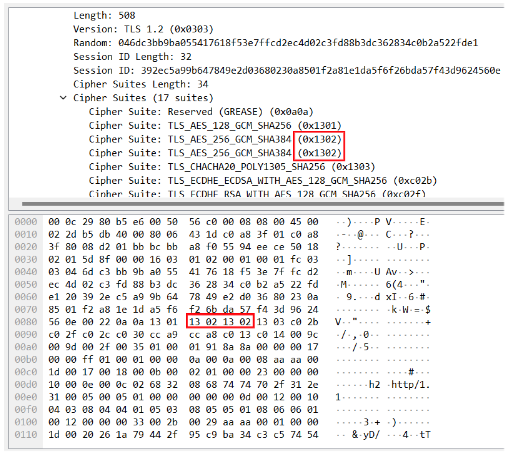
\includegraphics[width=\textwidth]{figures/cifrario_ripetuto.png}
	\caption{Pacchetto client hello inviato tramite Microsoft Edge}
	\label{cifrario_ripetuto}
\end{figure}

Nonostante i cifrari utilizzati siano uguali in numero, questo delinea una differenza di comportamento tra Edge e Firefox agevolando quindi il loro riconoscimento. Inoltre, l'eliminazione del cifrario ripetuto porterebbe Edge ad una situazione uguale a quella di Chrome e Opera in quanto a numero di cifrari, rendendoli quindi indistinguibili: l'ordine dei cifrari e le altre caratteristiche, infatti, sarebbero a quel punto identiche.

Ciò è probabilmente dovuto al fatto che questi tre browser si basano tutti su Chromium \footnote{https://www.chromium.org/chromium-projects/}, un web browser open source sul quale essi sono basati. Per questa ragione sono stati esclusi dalla trattazione Brave e Vivaldi, anch'essi basati su Chromium, in quanto dopo essere stati analizzati non differivano rispetto a Chrome e Opera.
\\
In sintesi, si può affermare che tre dei cinque browser analizzati si possano distinguere utilizzando soltanto dal pacchetto client hello inviato durante l'handshake TLS nel seguente modo:
\begin{enumerate}
	\item L'assenza del GREASE implica l'utilizzo di Firefox.
	\item Il numero di cifrari supportati permette la distinzione di Safari.
	\item La ripetizione di un algoritmo per la firma digitale consente un'ulteriore elemento di distinzione di Safari.
	\item La presenza di un cifrario duplicato consente di individuare Edge.
	\item La differenza in numero algoritmi di hashing comporta una distinzione di Firefox e Safari rispetto ai tre browser rimanenti.
\end{enumerate}


 








